% Chapter 2

\chapter{Management Summary} % Main chapter title

\label{Management Summary} % For referencing the chapter elsewhere, use \ref{Chapter1} 

%----------------------------------------------------------------------------------------



%----------------------------------------------------------------------------------------

\section{Introduction}
This Master thesis project aims to improve the effectiveness of cyber intelligence production process in the real world by solving the volumetric problems which exists in cyber intelligence domain by implementing Design science research method and the artefact design is verified by the security experts in a Group support session. 
Along with artefact design and validation, a simulation was done for feasibility check and the outcome of the simulated system has been very positive according to the users. 

%----------------------------------------------------------------------------------------

\section{The problem }
The current status quo is that Cyber news or Cyber informations are being pushed via multiple media (RSS, Mail, Web, feeds etc) to multiple people in a scattered way, and manually interpreted, this causes a dilute and incomplete picture. 
Especially in a world where threats emerge in numbers and sophistication (1 billion Unique malware samples this year). 
This thesis aims to build a prototype artefact, for collecting and assessing cyber news data and transfer that in actionable and valuable data for security professionals for making better decisions, by making use of a Design Science Research method.
This will ensure that the organizations using similar Cyber Intel methods are getting actionable and relevant Cybernews when they use this prototype. 
By using the Intel from this prototype, the organizations are potentially made more aware of the ongoing and relevant threats complemented with advisory to take action compared to traditional procedure of scanning multiple sources and looking for certain relevant threats.(see figure \ref{fig:problem_exsum}).

\begin{figure}
\centering
    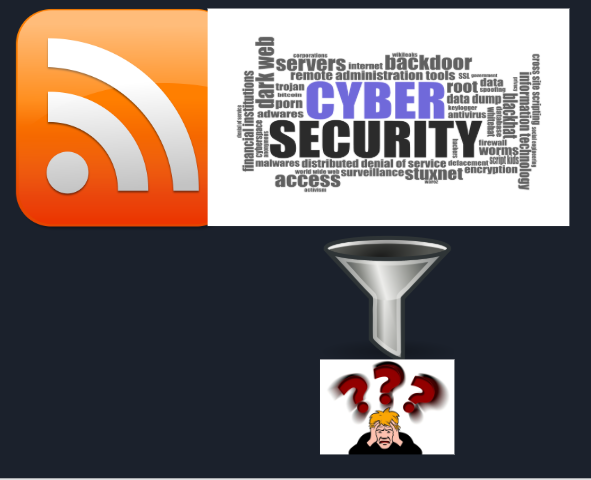
\includegraphics[scale=0.3]{Figures/problem}
    \caption{Problem of dealing with scattered information.}
    \label{fig:problem_exsum}
\end{figure}

%----------------------------------------------------------------------------------------

\section{The Solution Artefact prototype }
To design the artefact, a literature research was done on existing capability of the threat intelligence platforms and then the requirement need of an ideal system was explored with the users. The gaps found between the existing threat intelligence system and processes from the ideal system was addressed and a new artefact prototype by build and validated. 
\subsection{Prototype requirement and design}
We found that cyber information collection process is commonly available in almost every threat intelligence platforms. But it is important to add context and meaning to the cyber information so that it converts to cyber intelligence. For that:
\subsubsection{Requirement}
We need to add some extra algorithms and logics which could be implementable by a system for information filtering and tagging.
The data sources has to kept regularly sanitized with existing methods available.
The human intervention is needed for advisory so that the information is not only intelligent, it also becomes actionable.
\subsubsection{Solution design}
Based on the requirement and post assessment of 23 different tools, a solution prototype was build. This solution consist of system and processes required to transform a scattered information into cyber intelligence.

\subsection{Prototype Validation}
The solution build was validated with 6 experts in cyber security and 1 CEO of a Cyber security company. The overall solution was found to be, and  can be made available in market with some additional functional and technical capabilities.

\section{Conclusion }
The thesis turns to be truly successful and useful both in term of its academic purpose and practical use in real world problems. The main highlight of this thesis is a demo video with the academic concepts being implemented and can be visualised.







